\subsection{Linear structure, numerical reasoning, and uncertainty -- study additions}
\label{study-math}
\textit{AI-assisted editorial study additions: original explanations and illustrations, not verbatim historical writing nor a transcript. Calendar references guide subject scope, not claims of enrolment or completion.}

\subsubsection{Linear algebra as geometry and a computational tool}
For a linear map $A$, an eigenvector satisfies $Av=\lambda v$: its direction survives the transformation. Eigenvalues describe natural modes, but eigenvectors need not span the space. A defective matrix requires more than ordinary diagonalization. Real symmetric matrices are especially useful: an orthonormal eigenbasis exists, and the Rayleigh quotient $v^TAv/(v^Tv)$ lies between the smallest and largest eigenvalues. Positive eigenvalues then characterize a positive-definite quadratic energy.

The singular value decomposition works even for rectangular matrices:
\begin{equation}
A=U\Sigma V^T,\qquad Av_i=\sigma_i u_i,\qquad
\|A\|_2=\sigma_{\max}.
\label{study-math-svd}
\end{equation}
The right singular vectors identify input directions; singular values measure stretching; left singular vectors identify output directions. They are not generally eigenvectors. For $A=\left(\begin{smallmatrix}2&1\\1&2\end{smallmatrix}\right)$, the diagonal directions have eigenvalues and singular values $3$ and $1$. Truncating small singular values gives a low-rank approximation, but a threshold is a modelling decision tied to noise and resolution, not proof that nature has exactly that rank.
\begin{figure}[htbp]
\centering
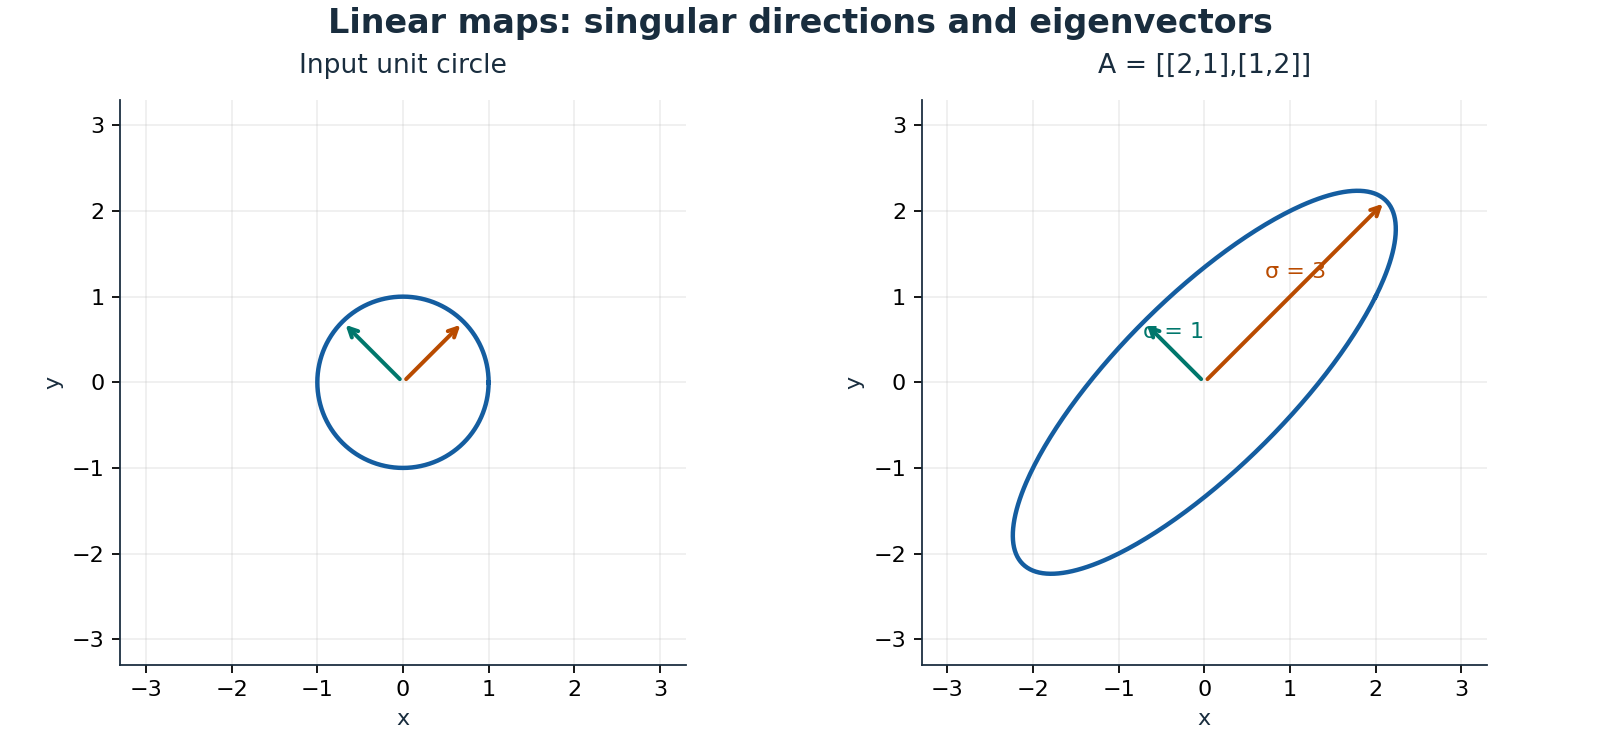
\includegraphics[width=0.95\linewidth]{tex_images/mental_map/study/math_svd.png}
\caption{A unit circle becomes an ellipse under a symmetric positive-definite map. The drawn directions have stretches three and one; the coincidence of eigenvectors and singular directions is special to this example.}
\label{study-fig-math-svd}
\end{figure}

For overdetermined measurements $Ax\approx b$, minimize $\|Ax-b\|_2^2$. Differentiation gives $A^T(A\hat x-b)=0$: the residual is orthogonal to the fitted column space. For measurements $(0,1),(1,2),(2,2)$, fitting an intercept and slope gives $\hat b=7/6$, $\hat m=1/2$, with residuals $(-1/6,1/3,-1/6)$. Their sum and their predictor-weighted sum vanish. Orthogonality does not establish that a straight line is scientifically appropriate.
\begin{figure}[htbp]
\centering
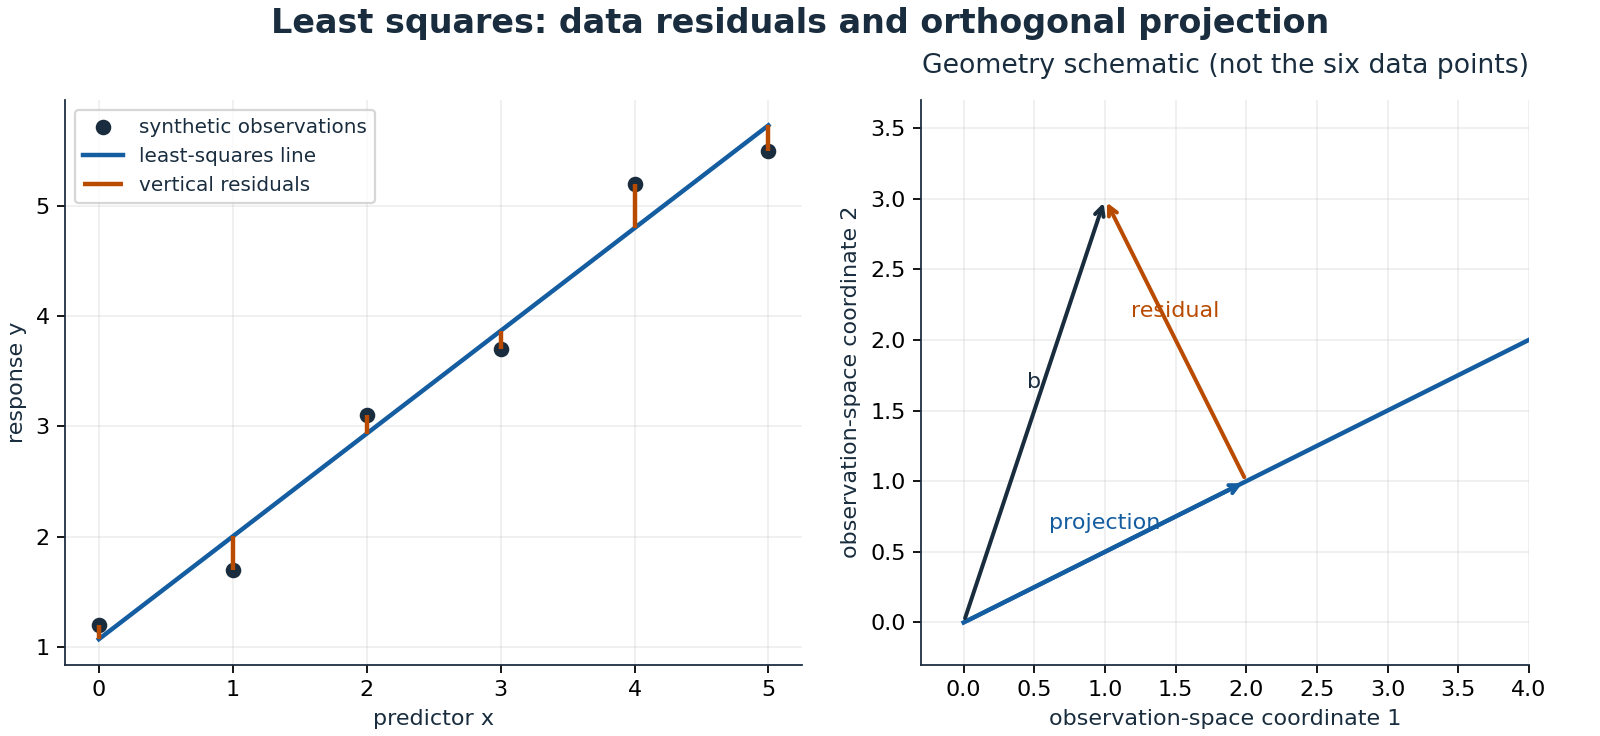
\includegraphics[width=0.95\linewidth]{tex_images/mental_map/study/math_least_squares.png}
\caption{Synthetic regression data show vertical residuals; the separate two-dimensional schematic shows orthogonal projection in observation space. It is not a geometric plot of the six-dimensional regression residual.}
\end{figure}

\subsubsection{Conditioning, local approximations, and numerical evolution}
Conditioning belongs to the problem; stability belongs to the algorithm. For nonsingular $A$, $\kappa_2(A)=\sigma_{\max}/\sigma_{\min}$ measures worst-case relative error amplification. Nearly parallel columns make fitted coefficients sensitive even when predictions barely change. Solving normal equations squares the condition number, so use QR or SVD rather than explicitly forming $(A^TA)^{-1}$. Scale quantities sensibly and report uncertainty rather than displaying unjustified digits.

Taylor expansion $f(x+h)=f(x)+hf'(x)+O(h^2)$ supplies a local error model, not a global guarantee. Newton's update
\begin{equation}
x_{k+1}=x_k-\frac{f(x_k)}{f'(x_k)}
\label{study-math-newton}
\end{equation}
sets a tangent approximation to zero. For $f(x)=x^2-2$ starting at $2$, the next iterates are $1.5$ and $17/12$. Local quadratic convergence needs a sufficiently close starting point, a simple root, and smoothness. A small derivative, multiple root, or distant initial guess can spoil it. Bracketing a continuous sign change gives bisection a slower but stronger guarantee. Terminate using residual and step criteria, scaled to the application's units.
\begin{figure}[htbp]
\centering
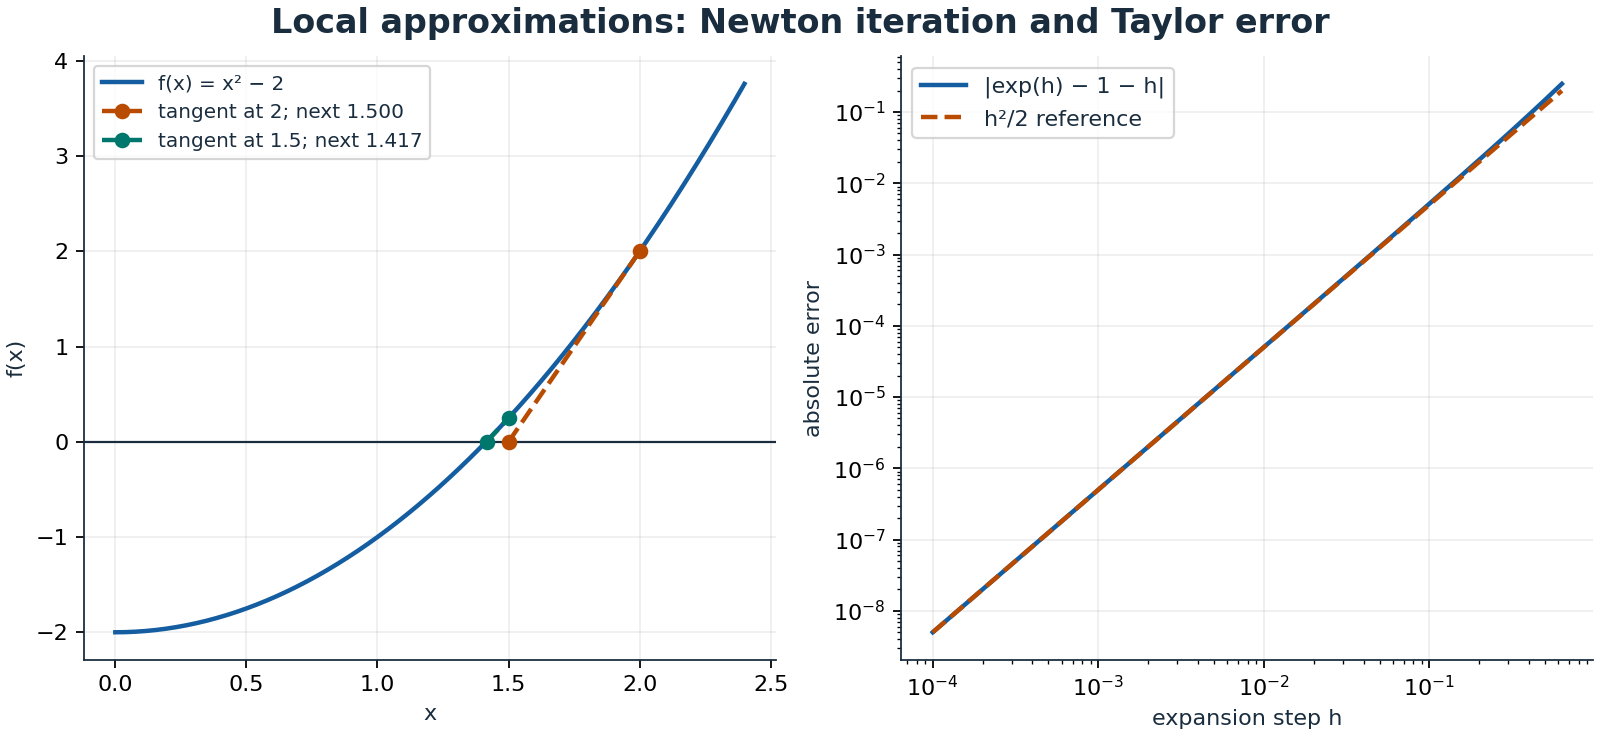
\includegraphics[width=0.95\linewidth]{tex_images/mental_map/study/math_newton.png}
\caption{Newton tangents for a square-root problem and the error of the first-order exponential approximation. The quadratic reference describes small steps, not arbitrary extrapolation.}
\end{figure}

Forward Euler advances $y_{n+1}=y_n+hf(t_n,y_n)$. Its local truncation error is $O(h^2)$ and typical fixed-interval global error is $O(h)$ under regularity assumptions. For $y'=-2y$, amplification is $1-2h$, so absolute stability requires $0<h<1$. A step of $0.8$ decays while alternating sign: numerically stable does not mean physically faithful. At $h=1.1$ it grows. Stiff equations can impose severe explicit-step limits; implicit methods trade solves for a larger stability region. Compare successive resolutions, conserved quantities, and an analytic case before trusting a simulation.
\begin{figure}[htbp]
\centering
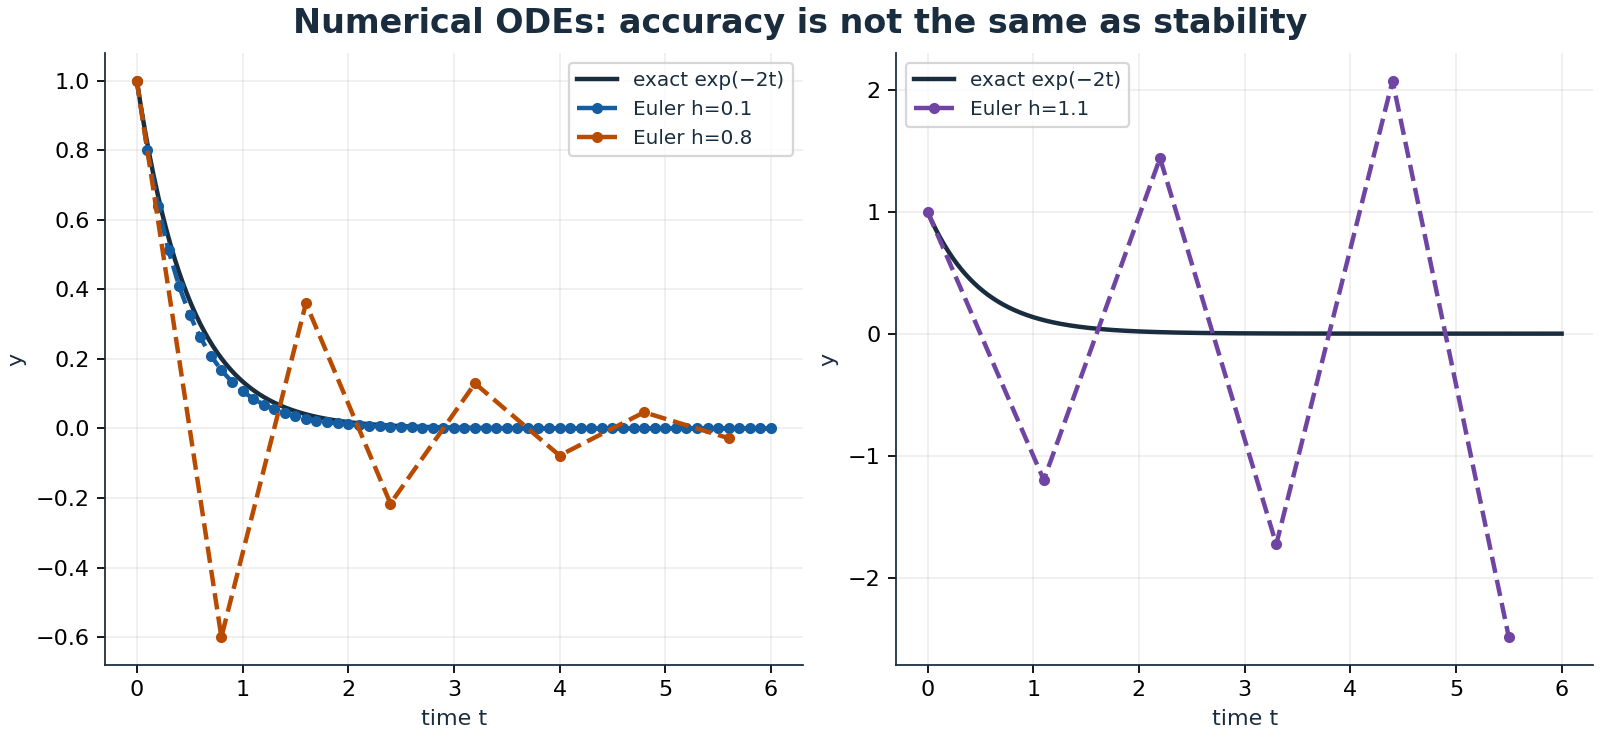
\includegraphics[width=0.95\linewidth]{tex_images/mental_map/study/math_ode.png}
\caption{Euler solutions of a dimensionless decay equation, with exact initial value one. A coarse stable step oscillates spuriously; a step beyond the stability boundary grows despite physical decay.}
\end{figure}

\subsubsection{Probability, estimation, and honest uncertainty}
A random variable models variation; an estimator is a rule applied to samples. Independent identically distributed observations with variance $\sigma^2$ give $\operatorname{Var}(\bar X)=\sigma^2/n$. The standard deviation describes individual spread; the standard error describes precision of an estimated mean. Correlation reduces effective information, and repeated measurements do not average away a shared calibration error. Bias, missingness, selection, and model mismatch require separate investigation.

A frequentist confidence interval is produced by a procedure with repeated-sampling coverage, not automatically a probability distribution for a fixed parameter. A Bayesian credible interval requires a likelihood and prior. For smooth $g$ and a covariance matrix $\Sigma$, first-order propagation gives $\operatorname{Var}(g(X))\approx\nabla g^T\Sigma\nabla g$. Retain covariance terms; independence cannot be inferred from separate column names. Report measurement units, sample selection, interval meaning, and assumptions together.
\begin{figure}[htbp]
\centering
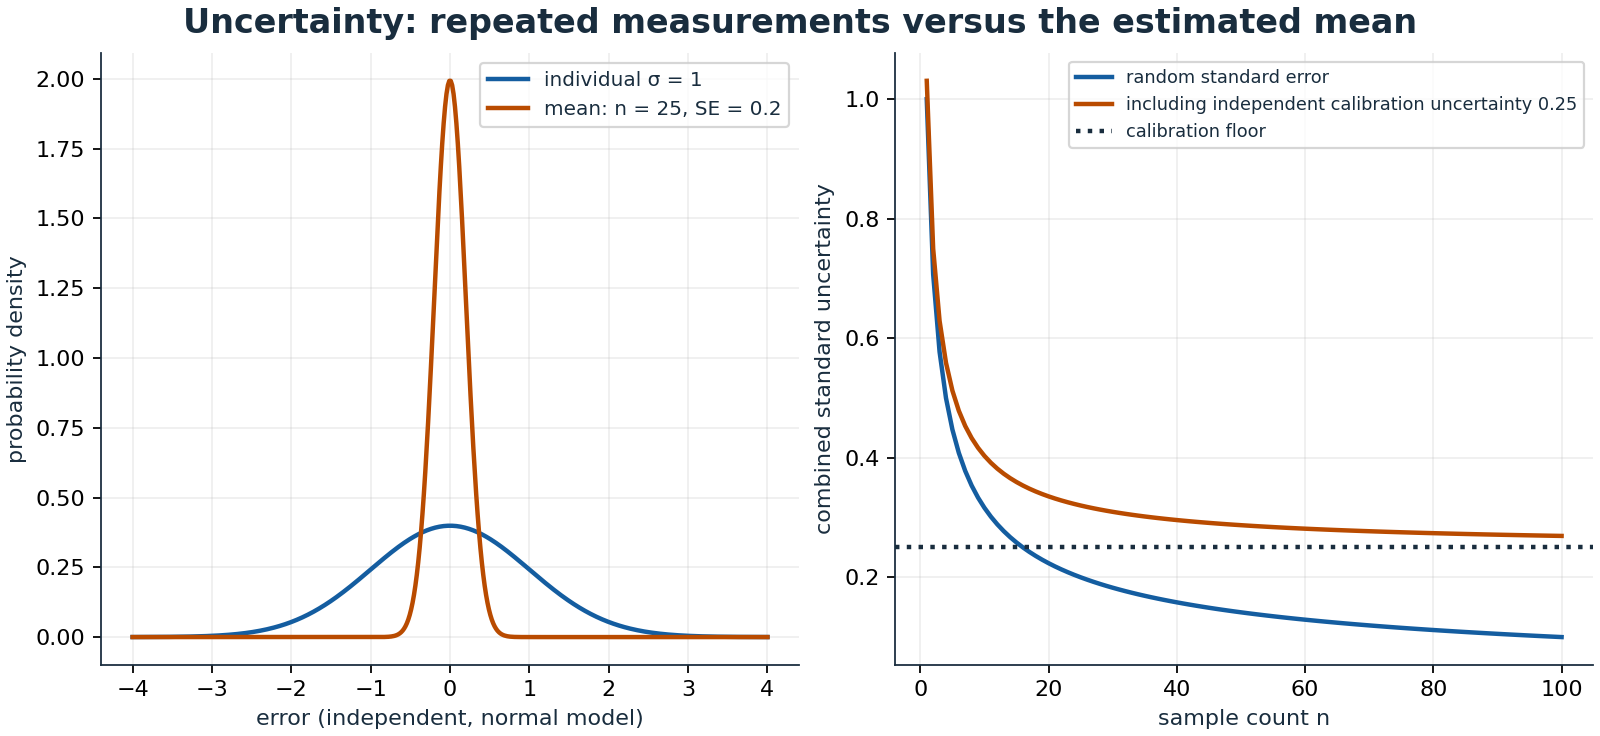
\includegraphics[width=0.95\linewidth]{tex_images/mental_map/study/math_uncertainty.png}
\caption{Normal-model individual and sample-mean distributions, plus an independent calibration uncertainty floor combined in quadrature. All curves are theoretical, not experimental confidence statements.}
\end{figure}

\subsubsection{Fields, boundaries, and transforms}
The gradient points toward greatest scalar increase; divergence measures local outward flux density; curl measures local circulation. Under suitable smoothness and orientation,
\begin{align}
\int_V\nabla\cdot F\,dV&=\int_{\partial V}F\cdot n\,dS,\label{study-math-gauss}\\
\int_S(\nabla\times F)\cdot n\,dS&=\oint_{\partial S}F\cdot d\ell.\label{study-math-stokes}
\end{align}
Gauss uses an outward closed-surface normal; Stokes pairs a surface normal with the right-hand boundary orientation. A field may circulate without diverging. Singularities and excluded holes require care before replacing integral information with a local derivative.
\begin{figure}[htbp]
\centering
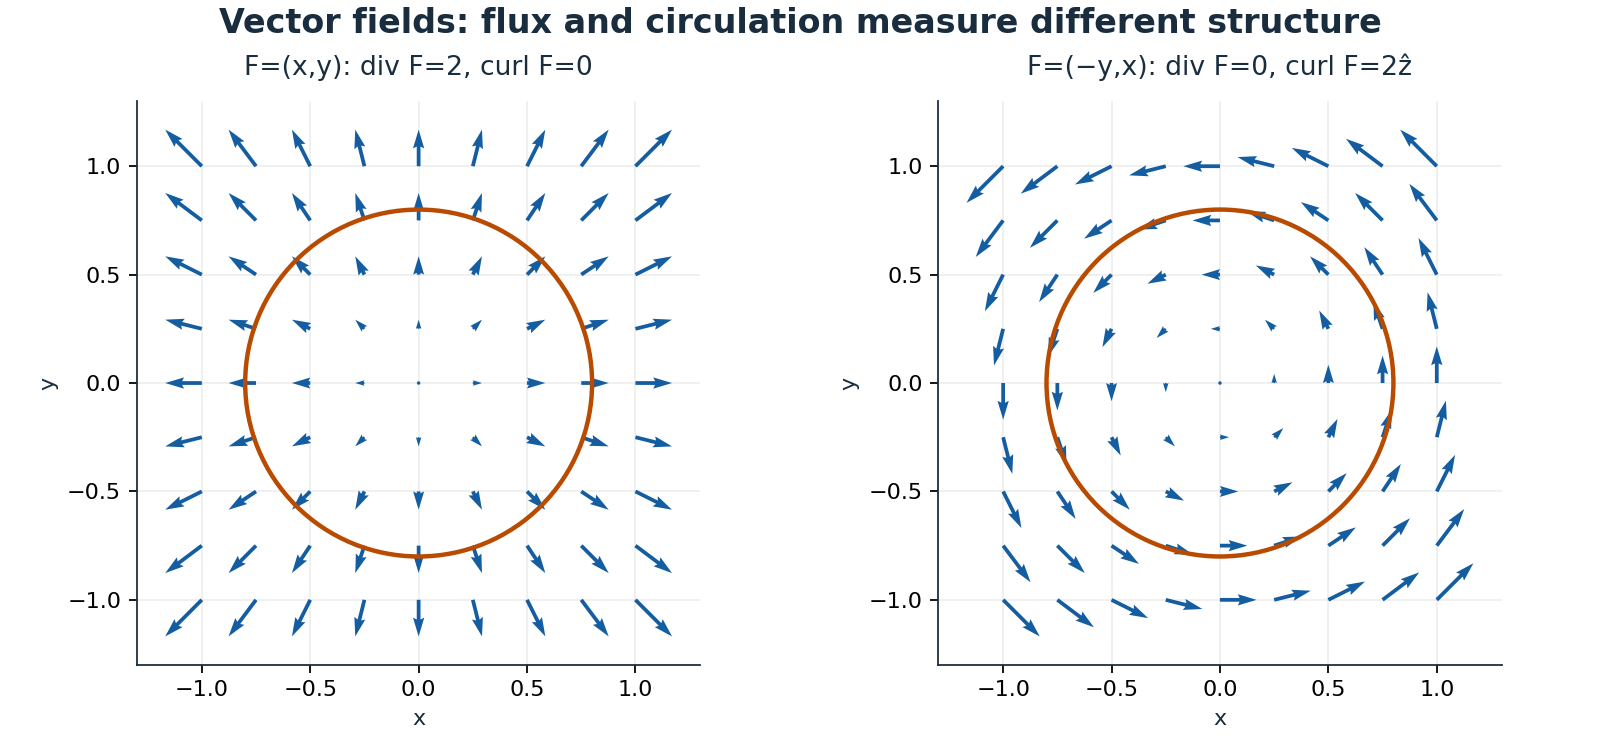
\includegraphics[width=0.95\linewidth]{tex_images/mental_map/study/math_fields.png}
\caption{Two smooth planar fields evaluated on a common grid. The circle is an integration boundary: radial expansion carries flux, while rigid rotation carries circulation.}
\end{figure}

The Laplace transform $F(s)=\int_0^\infty e^{-st}f(t)\,dt$ turns differentiation into $sF(s)-f(0)$ where the integral converges. Initial conditions matter; transfer functions normally describe zero-initial-condition response. Fourier analysis resolves oscillations into frequency components, with transform convention and normalization stated explicitly. A square wave has odd sine coefficients $4/(\pi k)$; truncation leaves Gibbs overshoot near jumps. More terms narrow the affected region rather than eliminating its limiting relative overshoot. Sampling additionally demands bandwidth control to prevent aliasing. These ideas connect directly to feedback in Section~\ref{study-control} and diffusion in Section~\ref{study-physics}.
\begin{figure}[htbp]
\centering
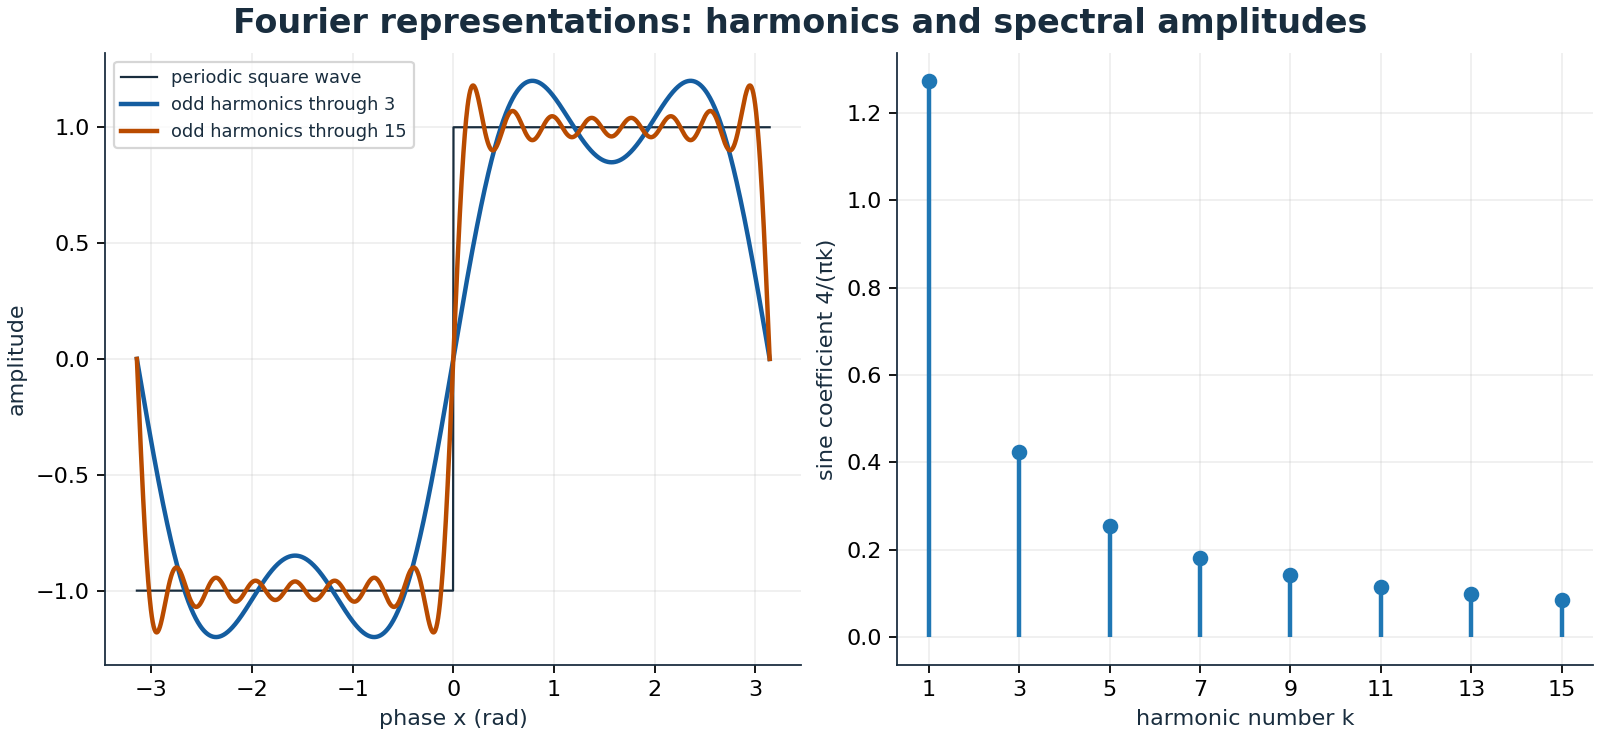
\includegraphics[width=0.95\linewidth]{tex_images/mental_map/study/math_fourier.png}
\caption{Odd-harmonic approximations to a periodic square wave and their sine coefficients. Endpoint values are convention-dependent; the displayed finite sums show persistent near-jump overshoot.}
\end{figure}

\subsubsection{Scope and further study}
The \href{https://ucalendar.uwaterloo.ca/2223/COURSE/course-NE.html}{Waterloo 2022/23 NE calendar} motivates linear algebra, probability, numerical methods, and vector calculus through NE 112, 113, 215, 216, and 217. The \href{https://ucalendar.uwaterloo.ca/2223/COURSE/course-SYDE.html}{SYDE calendar} supplies additional scope, including SYDE 312. Neither establishes personal attendance. For independent explanations and exercises, see \href{https://ocw.mit.edu/courses/18-06-linear-algebra-spring-2010/}{MIT OpenCourseWare: Linear Algebra}.